%%%%%%%%%%%%%%%%%%%%%%%%%%%%%%%%%%%%%%%%%%%%%%%%%%%%%%%%%%%%%%%%%%%%
\section{Interfaces} % (3 pages)} 
\label{sec:fdsp-apa-intfc}

The interface between the APA consortium and other detector consortia, facilities, and working groups
covers a wide range of activities. Table~\ref{tab:apa_interface_docdb} summarizes the interface control
documents being developed. In the following, we elaborate on three relatively important
interfaces: electronics, photon detectors, and the high voltage system. 

\begin{dunetable}[APA interface control documents]{lr}{tab:apa_interface_docdb}
{Summary of interface control documents being developed.}  
  Interface Document & DUNE doc-db number \\\hline
  Interface to TPC electronics & 6670 \\ 
  Interface to photon detector system & 6667 \\
  Interface to drift high voltage system & 6673 \\
  Interface to DAQ & 6676 \\
  Interface to slow controls and cryogenics infrastructure & 6679 \\\hline
  Integration facility interface & 7021 \\
  Facility interfaces (Detector Hall, Cryostat, and Cryogenics) & 6967 \\
  Installation interface & 6994 \\
  Calibration interface & 7048 \\\hline
  Software computing interface & 7102 \\
  Physics interface & 7075 \\
\end{dunetable}


%%%%%%%%%%%%%%%%%%%%%%%%%%%%%%%%%
\subsection{TPC Cold Electronics}
\label{sec:fdsp-apa-intfc-elec}

The TPC readout electronics are directly mounted on the APA immersed inside LAr in order to reduce the input capacitance and thus the inherent electronics noise, hence cold electronics (CE).  With the wire-wrapped design, all 2,560 wires to be read out (960 are G-plane wires intended for charge shielding only and not connected to readout electronics) are terminated on wire boards that stack along one end (the head) of the APA frame.  Ten such stacks of wire boards, pinned for readout, are installed across the width of each side of the frame. There are a total of 128 readout channels (48/40/40 for X/U/V) in each stack. The 2,560 channels per APA are, therefore, read out by 20 front-end motherboards (FEMBs), each of which includes eight 16-channel front-end ASICs, eight 16-channel ADC ASICs, low-voltage regulators, and input signal protection circuits.  A schematic view of the head end of an APA with electronics installed and a cable tray mounted above is shown in Fig.~\ref{fig:apa_ce}. 

\begin{dunefigure}[APA electronics interface]{fig:apa_ce}
{The head region of an APA frame showing the 10 wire board stacks on each side, 20 front-end motherboard boxes, and the cable tray mounted above.}
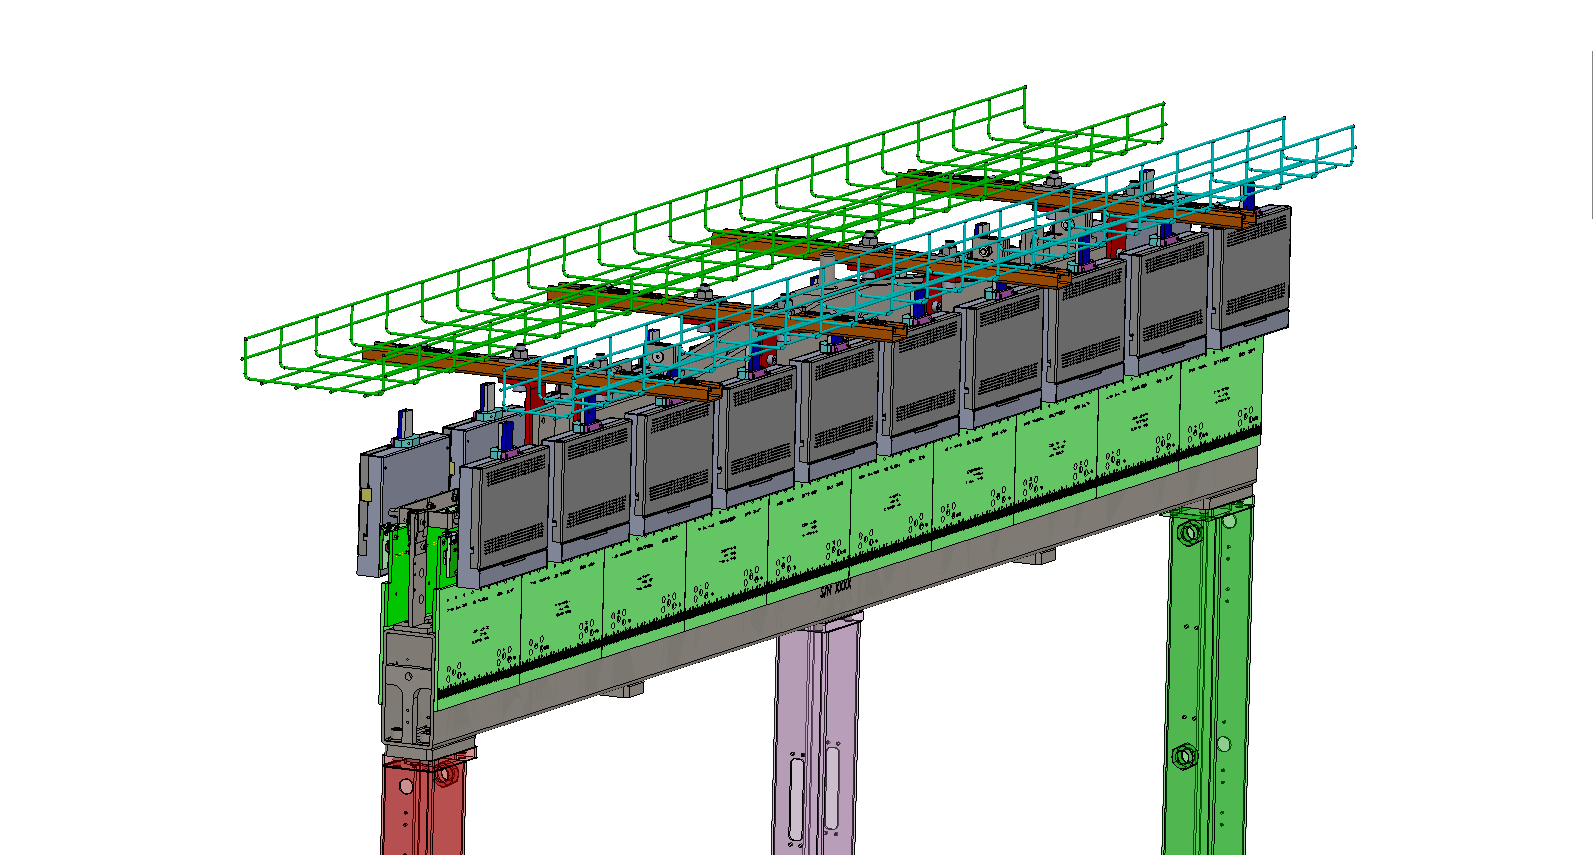
\includegraphics[width=0.8\textwidth,trim=10mm 0mm 10mm 20mm, clip]{APA_interface.png}
\end{dunefigure}

The interface between the APA and TPC cold electronics covers a wide range of topics, including the hardware design and production, testing, integration, installation, and commissioning. The hardware interface basically has two components, mechanical and electrical. The mechanical interface includes the support of the 20 CE boxes with each housing a FEMB. 

The electrical interface covers $i$) the choice of wire-bias voltages to the four wire planes so that 100\% transparency can be achieved for drifting ionization electrons, $ii$) cable connection for the wire bias voltages from the cryostat feedthroughs to the CR boards, $iii$) interface boards providing connection between CR boards and CE boxes, $iv$) filtering of the wire-bias voltages through CR boards in order to suppress potential introduction of electronics noise, and $v$) an overall grounding scheme and electrical isolation scheme for each APA. The last item is particularly important in order to reach the low electronics noise levels required.


%%%%%%%%%%%%%%%%%%%%%%%%%%%%%%%%%
\subsection{Photon Detection System}
\label{sec:fdsp-apa-intfc-pds}

While the design of the Photon Detector System (PDS) is still under development, it is expected that the PDS is integrated into the APA frame to form a single unit for the detection of both ionization charge and scintillation light. For the present baseline design, the PDS is expected to be installed into the APA frame at the integration test facility after the completion of the wire winding (see Section~\ref{sec:fdsp-apa-install}). Figure~\ref{fig:apa-pd} shows the final step in installing the PDS into the APA frame. The PDS signal cable connection is highlighted.  An alternative design of installing PDS elements prior to the wire winding is also under consideration. Similar to that of cold electronics, the interface between PDS and APA covers a wide range of topics, including the hardware design and production, testing, integration, installation, and commissioning. The hardware interface again includes two components: mechanical and electrical interfaces. The mechanical interface includes $i$) supports for the PDS detectors, $ii$) access slots for installation of the detectors, $iii$) access slots for the cabling of the detectors and routing of the PDS cables inside the beams of the APA frame. Depending on the final design of the PDS, the geometry of the APA, including the slot dimension and the number of slots, may require modification. Any proposed changes by the PDS Consortium must be evaluated by the APA Consortium to understand structural impacts or interferences with other components.

The electrical interface includes a grounding scheme and electrical insulation. Due to the strict requirements on the noise from the cold electronics (CE), the electrical interface must be defined together with the CE Consortium. In addition, an electrical test will be performed with a APA/PDS/CE vertical slice test. 

\begin{dunefigure}[APA interface with photon detectors]{fig:apa-pd}
{(Left) Installation of a photon detector module into the APA frame. The cable connection is highlighted. (Right) The baseline design for PDS cable routing. Photon detector cables are expected to go through the central beam and be distributed inside the supporting tubes of APA frame.}
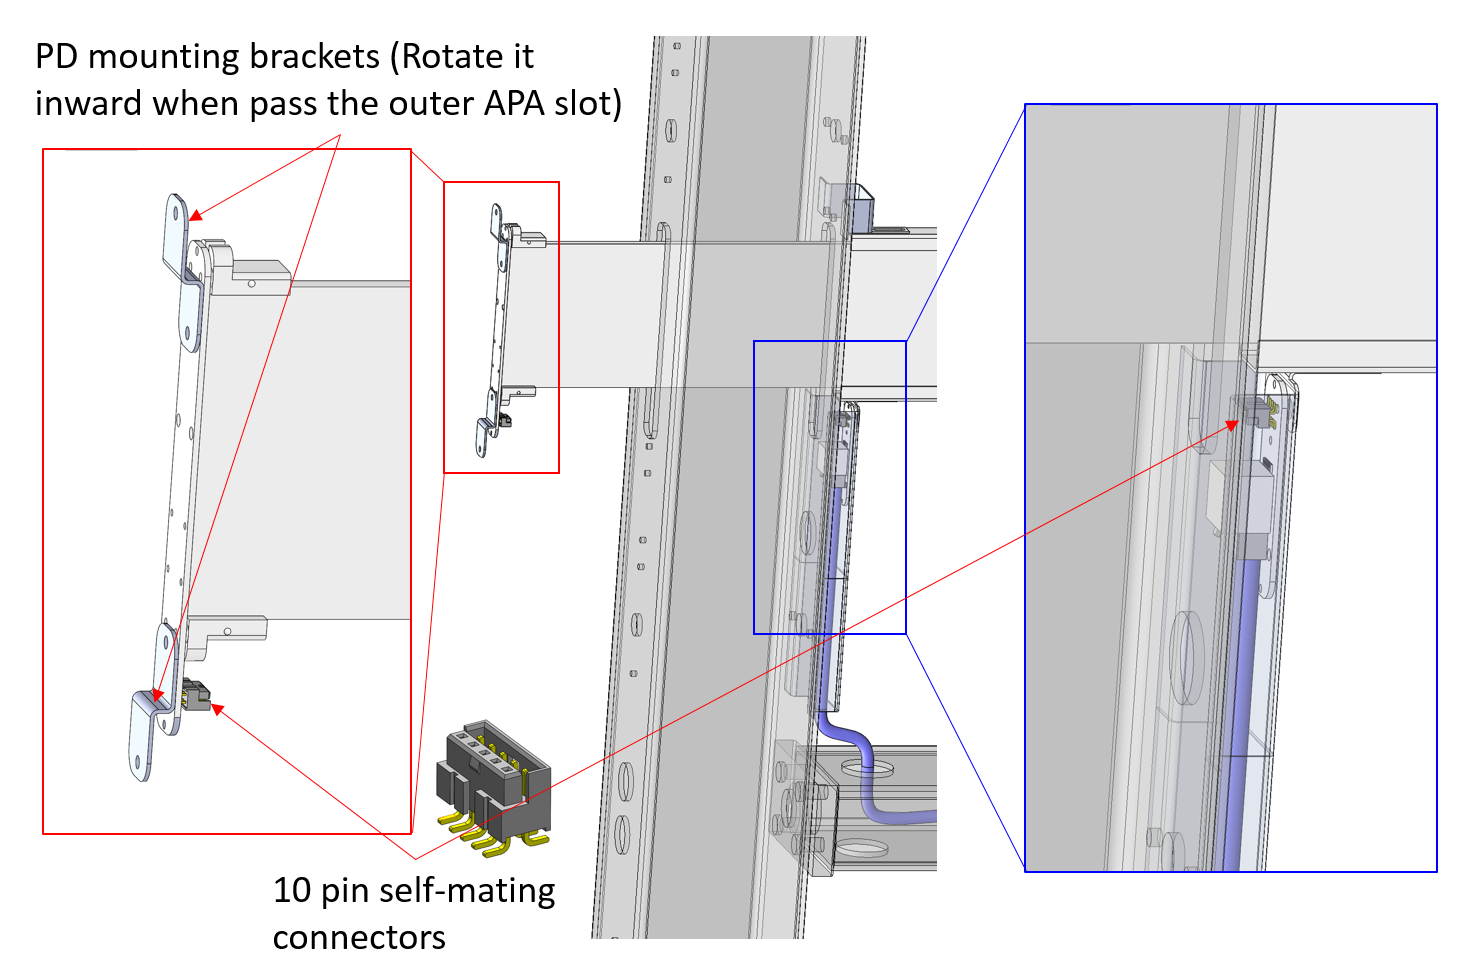
\includegraphics[height=0.3\textheight]{PD-APA2.PNG}
%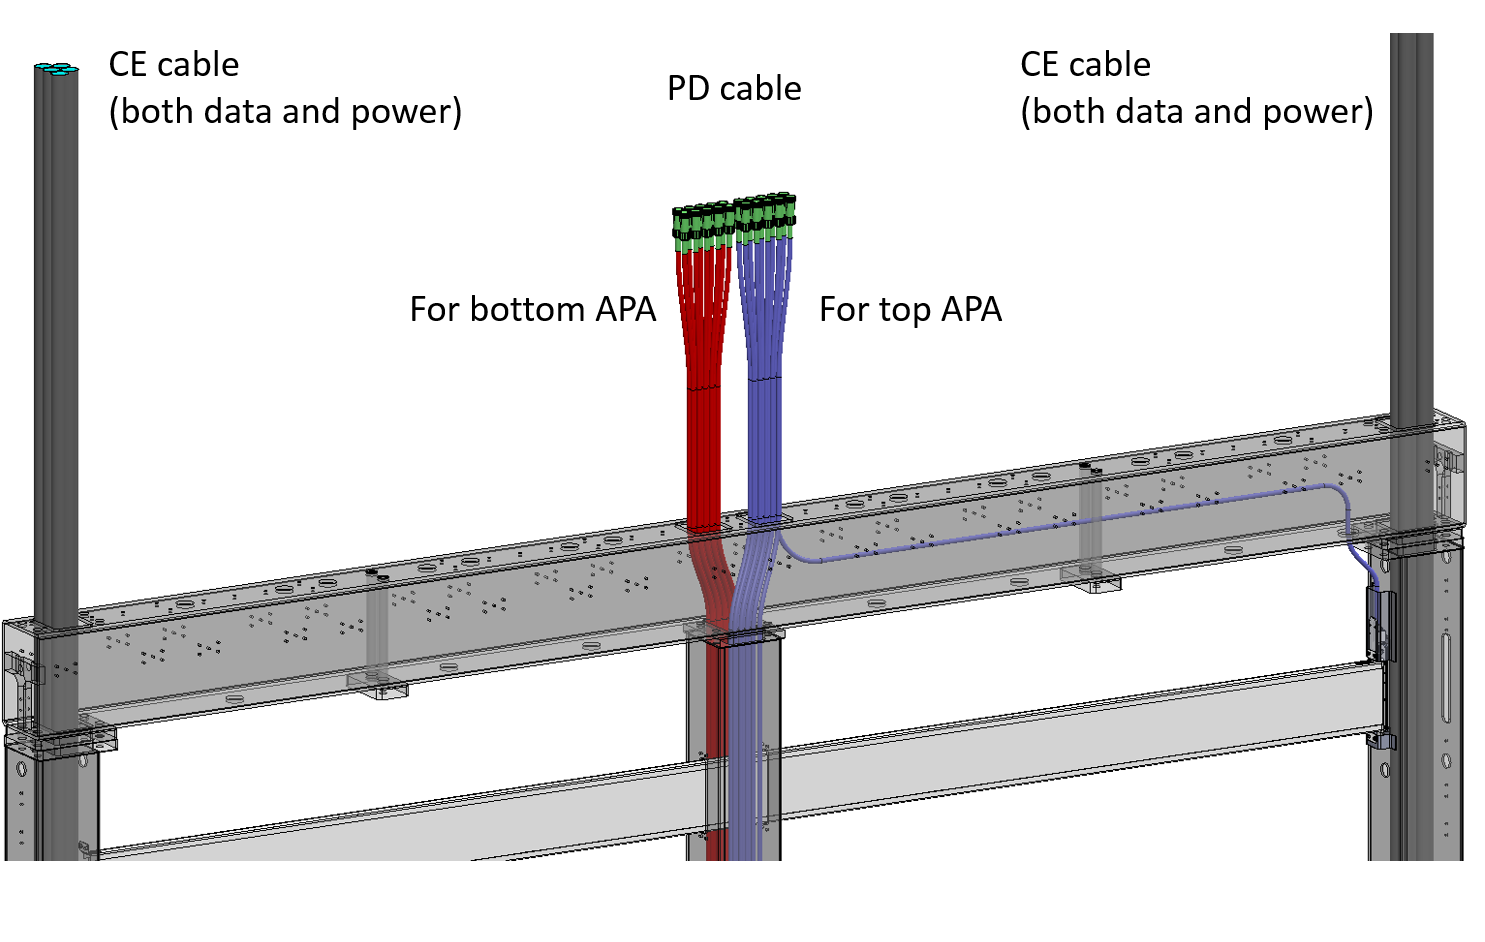
\includegraphics[height=0.23\textheight]{PD-APA1.PNG}
\end{dunefigure}


%%%%%%%%%%%%%%%%%%%%%%%%%%%%%%%%%
\subsection{APA to APA Connections and Cable Routing}

The TPC readout electronics require that the APA frames must be electrically isolated.  The left panel of Figure~\ref{fig:apa-cabling} shows the current conceptual design for mechanically connecting the two APAs in a vertical stack while maintaining electrical isolation.  The green elements are an insulating panel and sleeve made from G10. 

For the present baseline design, the cables of the PDS are expected to be routed inside the central beam of the APA frame.  The CE electrical cables need to be routed so that the head end of the lower APA in the 2-APA assembly can be reached. The default design is to rout the CE cables (power and signal) inside the two side beams of the APA frames. The right panel of Fig.~\ref{fig:apa-cabling} shows the baseline cable routing scheme.     

\begin{dunefigure}[APA-to-APA connection and cable routing]{fig:apa-cabling}
{(Left) Conceptual design for the APA-to-APA connection.  The green insulator pieces act to electrically isolate the two frames, as required by the front-end electronics.  (Right) The baseline design for PDS cable routing. Photon detector cables are expected to go through the central beam and be distributed inside the supporting tubes of APA frame.  CE cables (both data and power) go down the outside tubes to reach the lower APA.}
\setlength{\fboxsep}{0pt}
\setlength{\fboxrule}{0.5pt}
\fbox{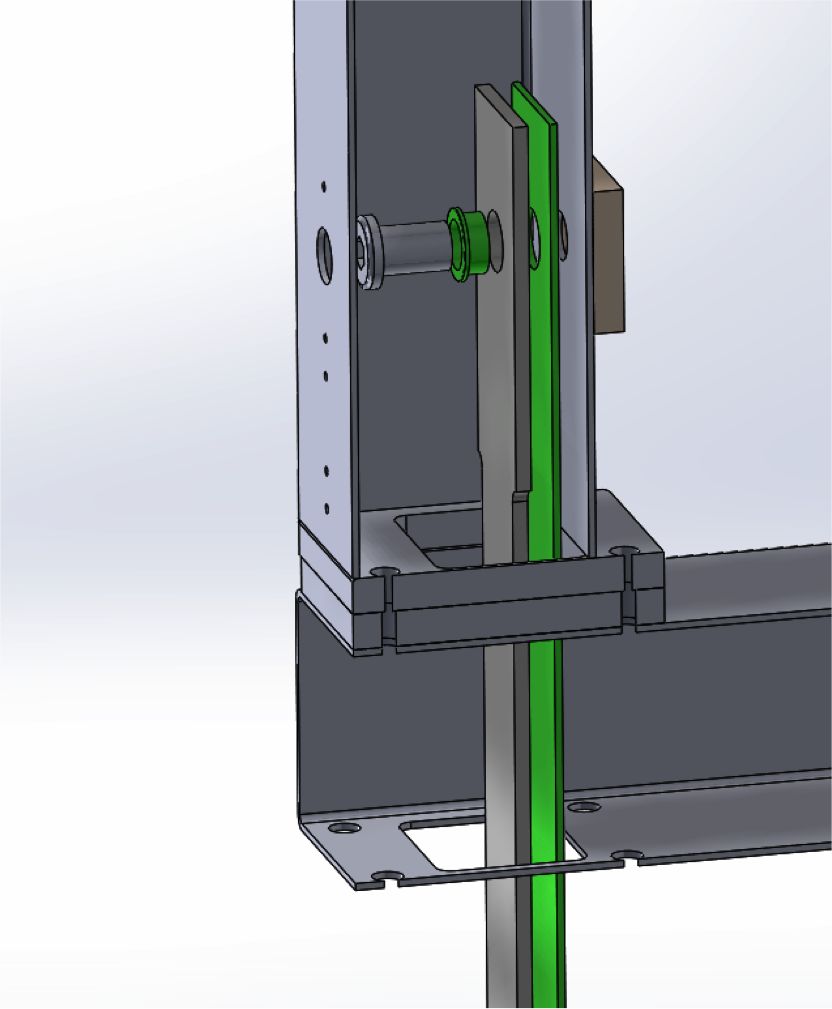
\includegraphics[height=0.27\textheight]{apa-apa-mating.png}}\qquad \quad
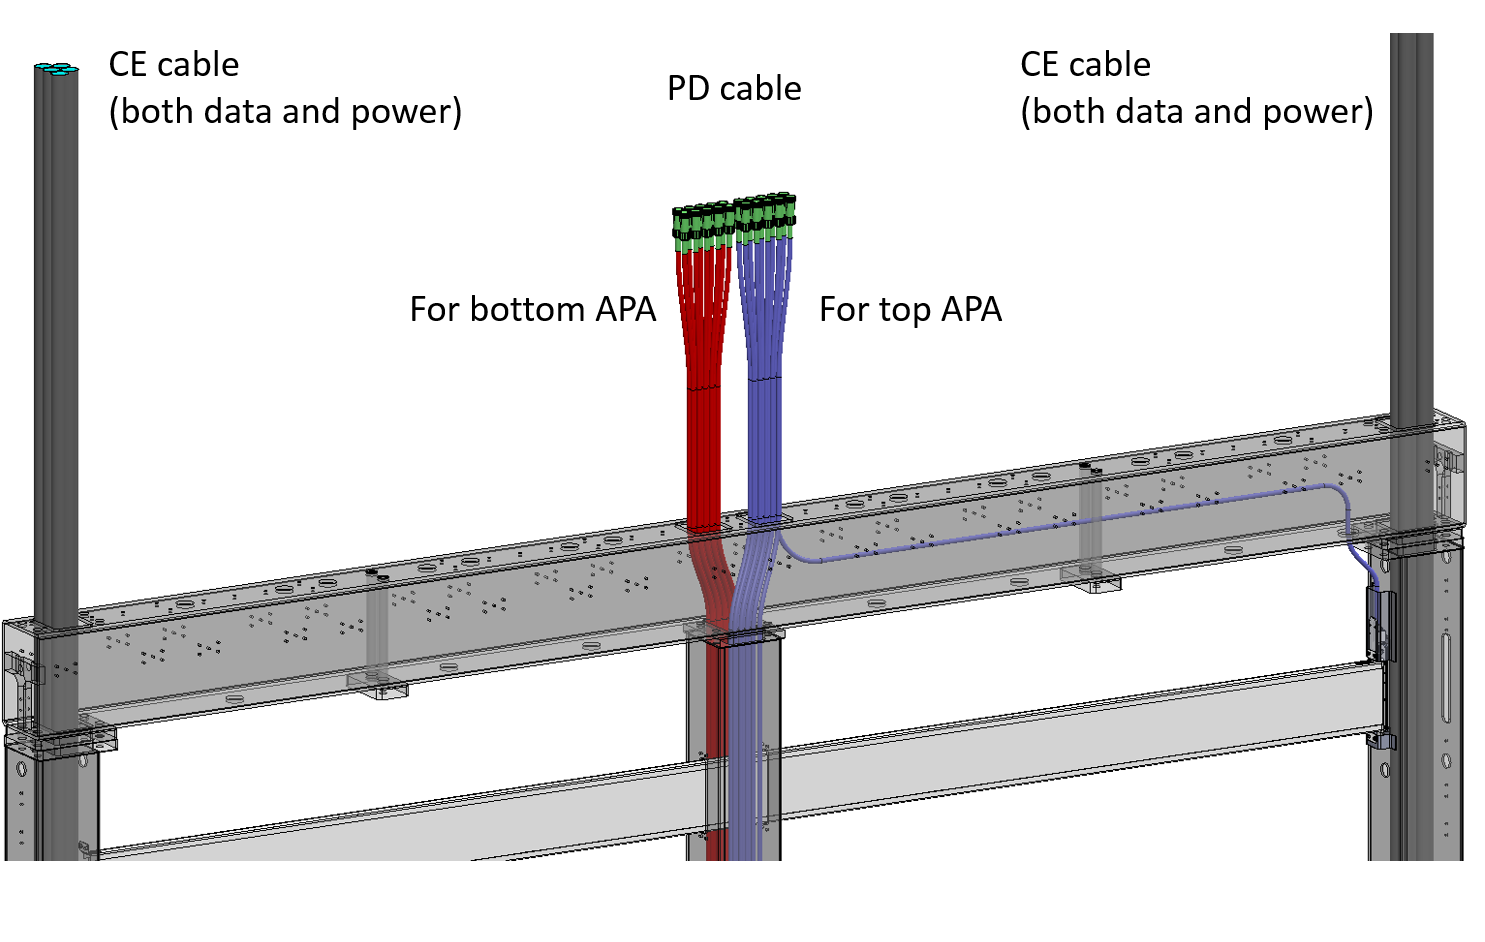
\includegraphics[height=0.27\textheight]{PD-APA1.PNG}
\end{dunefigure}

%%%%%%%%%%%%%%%%%%%%%%%%%%%%%%%%%
\subsection{High Voltage System}
\label{sec:fdsp-apa-intfc-hv}

\todo{Details left for the HV chapter, with  reference here}

%%%%%%%%%%%%%%%%%%%%%%%%%%%%%%%%%
\subsection{LBNF Cryostat and Detector Support Structure}
\label{sec:fdsp-apa-intfc-lbnf-dss}

\todo{Details left for the Technical Coordination chapter, with reference here}
